\chapter*{Annexe 2}
\addcontentsline{toc}{chapter}{Annexe 2}

%recommencer la numérotation des section à "1"
\setcounter{section}{0}

Intro

\section*{Prérequis}
\addcontentsline{toc}{section}{Prérequis}

Bla

\begin{itemize}
\item item1;
\item item2;
\item item3;
\item item4.
\end{itemize}

Bla

\section{Partie 1}

Bla

\subsection{Sous-parie 1}

Bla

\subsection{Sous-parie 2}

Bla

\section{Partie 2}

\begin{center}
\textsc{Attention !}

\textit{Texte d'avertissement}
\end{center}

Bla

\newpage

\section{Partie 3}

Bla

\begin{figure}[!ht]
\begin{center}
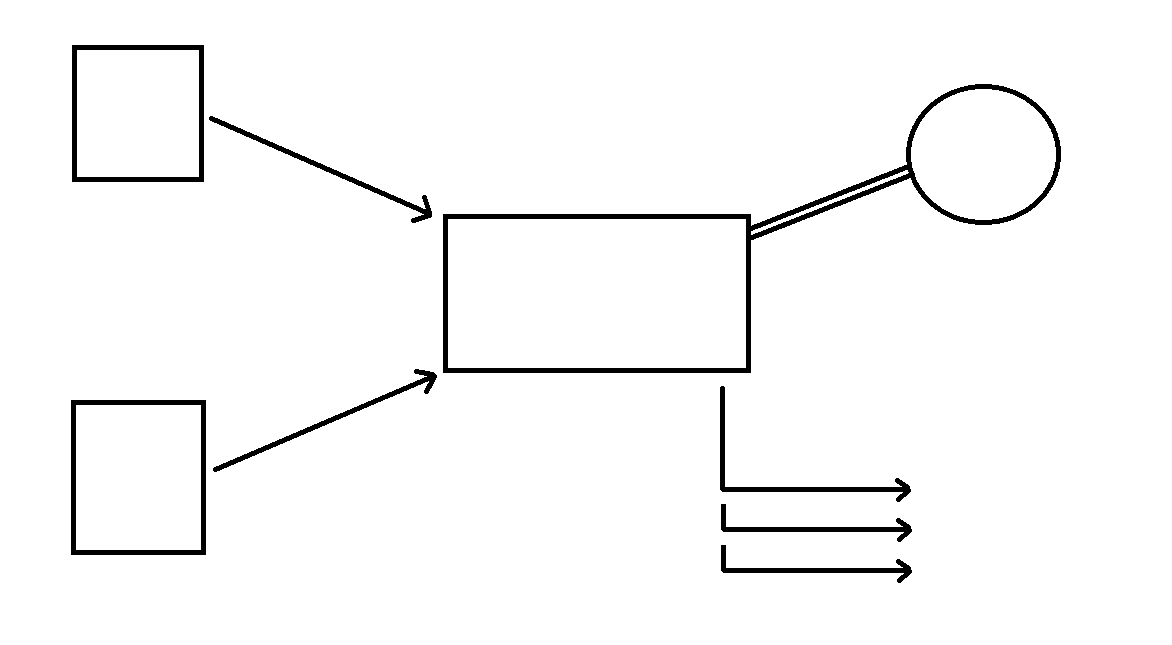
\includegraphics[height=8cm]{presentation/schema}
\end{center}
\caption[schema]{Presentation schema}
\end{figure}

\paragraph*{Paragraphe 1}
~\\
\hskip7mm

Bla

\paragraph*{Paragraphe 2}
~\\
\hskip7mm

Bla

\paragraph*{Paragraphe 3}
~\\
\hskip7mm

Bla